
\begin{figure}[!t]
    \centering
    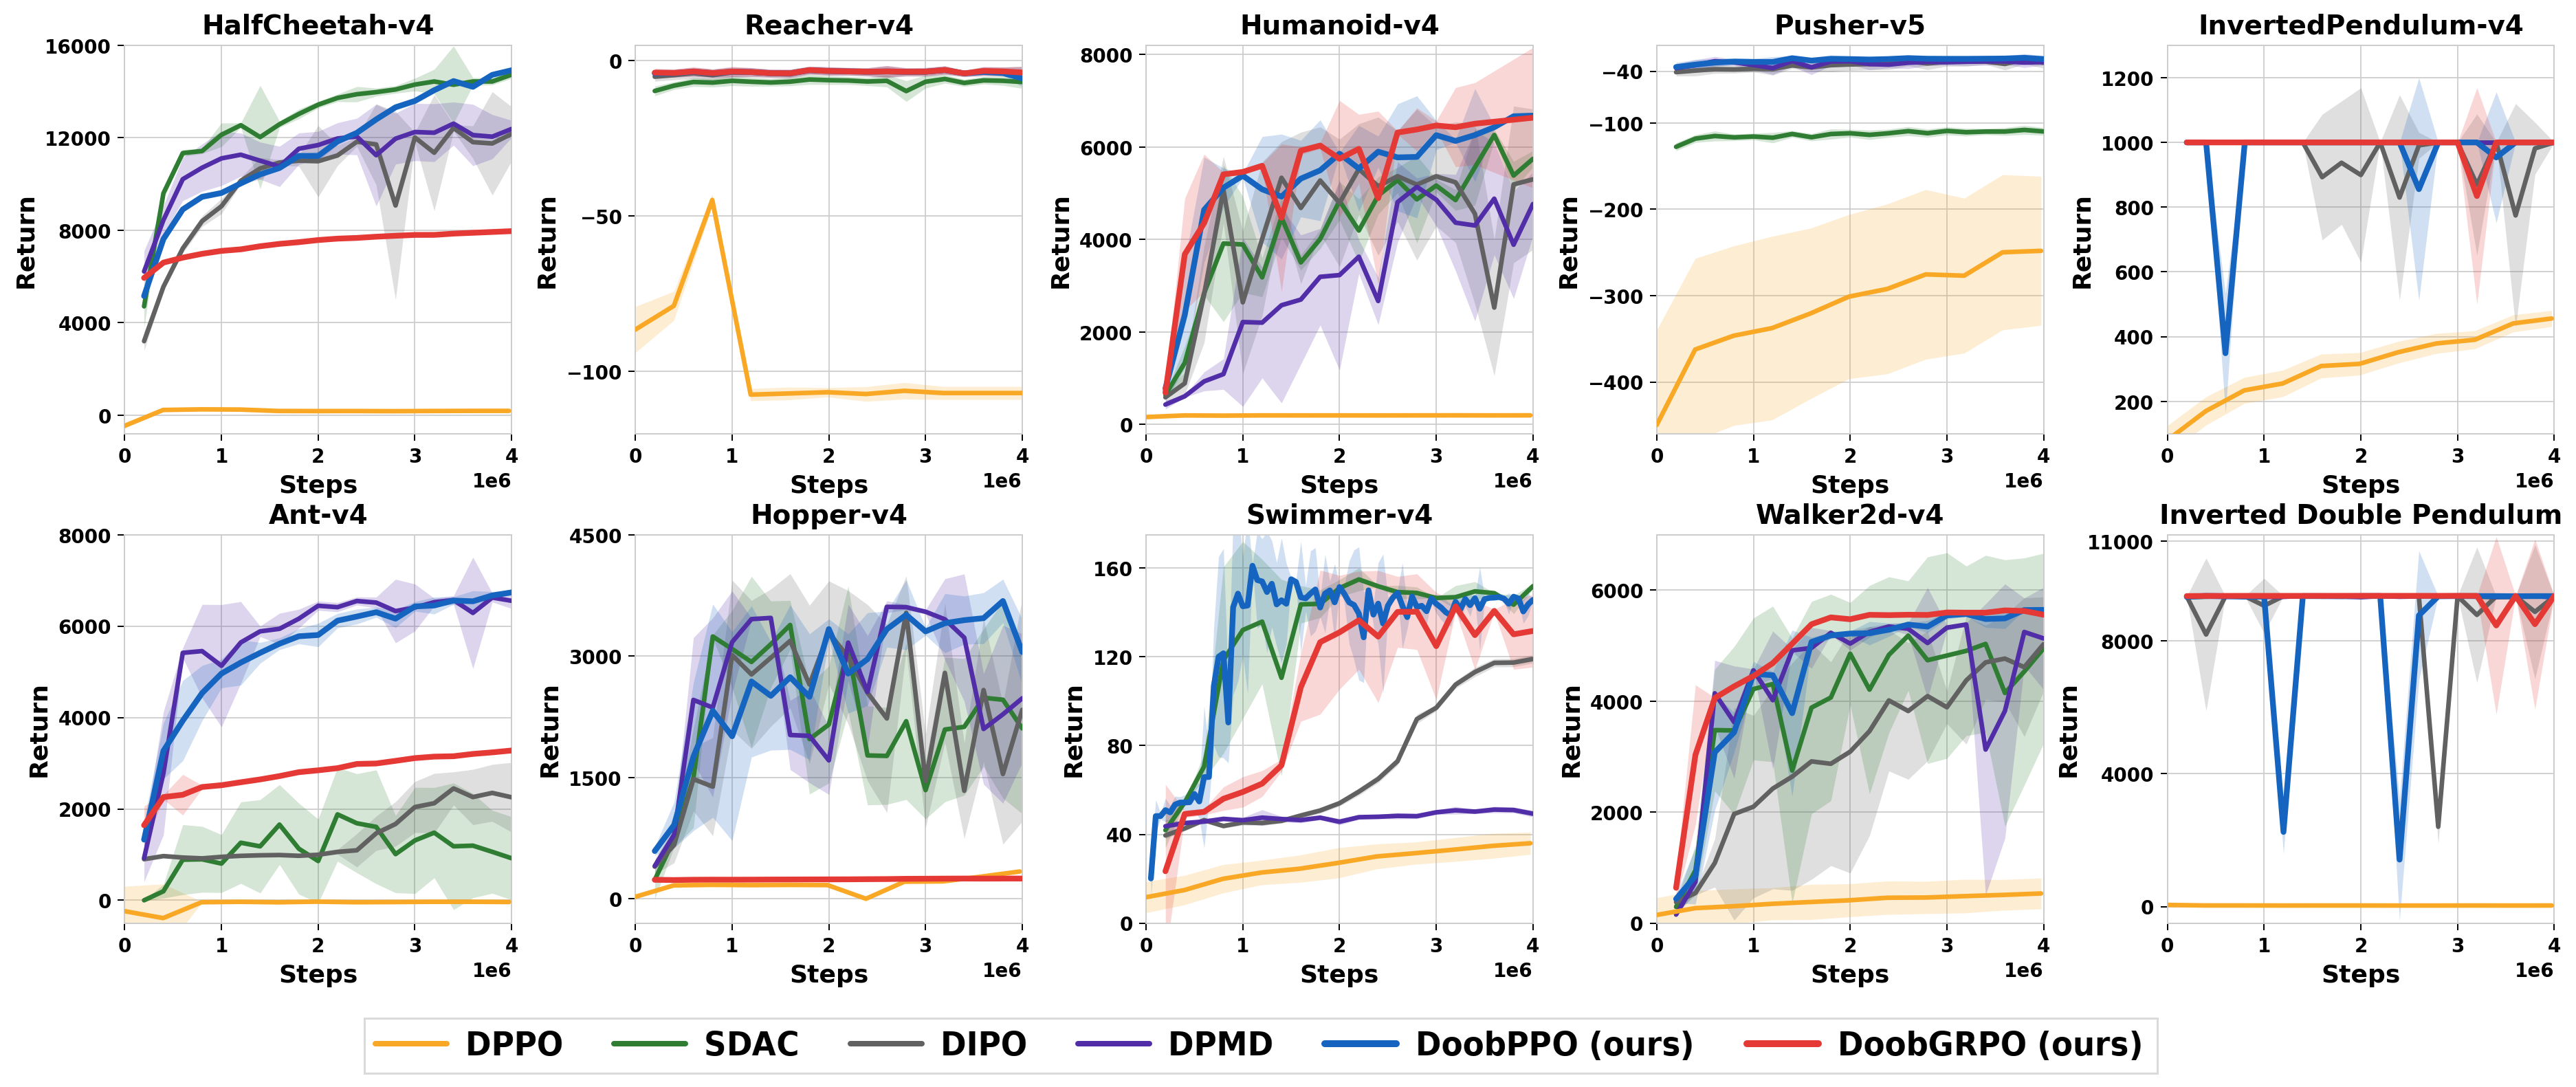
\includegraphics[width=1\linewidth]{mujoco10_4m_doob_grid.png}
    \caption{\small Learning curves on 10 MuJoCo continuous-control tasks, evaluated every 200k environment steps. Curves show mean undiscounted return over 3 training seeds, with shaded regions indicating one standard deviation. We compare DoobPO against strong diffusion-policy baselines DPPO, SDAC, DIPO, and DPMD.}
    \label{fig:mujoco10_dp}
\end{figure}

This section presents the experimental results.
We evaluate DoobPO on OpenAI Gym MuJoCo continuous-control benchmarks and on Robomimic manipulation tasks.
We describe the experimental setup in \cref{sec:exp_setup}.
We then report the results of RL fine-tuning diffusion and flow policies with DoobPO in \cref{sec:diffusion_exp} and \cref{sec:flow_exp}, and the Robomimic results in \cref{sec:robomimic_exp}.

\subsection{Experimental Setup}
\label{sec:exp_setup}

\textbf{Environments: OpenAI Gym MuJoCo.}
We evaluate our method on 10 OpenAI Gym MuJoCo continuous-control tasks covering locomotion, manipulation, and stabilization.
All diffusion-policy methods are trained from scratch for $4$M environment steps, while all flow-policy methods are trained from scratch for $5$M environment steps, under the same interaction budget within each setting.

\paragraph{Evaluation Metric.}
We use episode return as the evaluation metric, where higher return indicates better control performance.
During training, the policy is evaluated periodically, and at each evaluation point we report the mean return and its standard deviation over 3 random seeds.

\subsection{Diffusion Policy Comparison}
\label{sec:diffusion_exp}

\paragraph{Baselines.}
We compare DoobPO against recent diffusion-policy RL baselines, including DIPO \cite{yang2023policyrepresentationdiffusionprobability}, DPPO \cite{ren2024diffusion}, DPMD \cite{ma2025efficient}, DACER \cite{wang2024diffusionactorcriticentropyregulator}, and SDAC \cite{ma2025efficient}, as well as PPO \cite{schulman2017proximal}, TRPO \cite{schulman2015trust}, and SAC \cite{haarnoja2018soft}.
Please see \cref{sec:related_works} for details.

\begin{table*}[t]
\centering
\small
\setlength{\tabcolsep}{3.5pt}
\renewcommand{\arraystretch}{0.95}
\caption{\small Diffusion Policy Performance on MuJoCo environments
(mean $\pm$ std over 3 random seeds).
The best results are in bold and the second-best results are underlined.}
\label{tab:mujoco_grouped}
\begin{adjustbox}{max width=\textwidth}
\resizebox{0.9\linewidth}{!}{%
\begin{tabular}{llccccc}
\toprule
& Method
& HalfCheetah
& Reacher
& Humanoid
& Pusher
& InvertedPendulum \\
\midrule

\multirow{3}{*}{\textbf{Classic Model-Free RL}}
& PPO
& 1696 $\pm$ 223
& -3.63 $\pm$ 1.54
& 492 $\pm$ 113
& -25.28 $\pm$ 2.73
& \textbf{1000 $\pm$ 0} \\

& TRPO
& 2941 $\pm$ 417
& -3.83 $\pm$ 1.89
& 440 $\pm$ 82
& -31.84 $\pm$ 6.32
& \textbf{1000 $\pm$ 0} \\

& SAC
& 14422 $\pm$ 20
& -3.03 $\pm$ 1.21
& 5866 $\pm$ 16
& -23.96 $\pm$ 3.47
& \textbf{1000 $\pm$ 0} \\

\midrule

\multirow{7}{*}{\textbf{Diffusion Policy RL}}
& DIPO
& 12169 $\pm$ 1172
& -3.09 $\pm$ 1.36
& 5523 $\pm$ 980
& -27.85 $\pm$ 2.08
& \textbf{1000 $\pm$ 0} \\

& DPPO
& 248 $\pm$ 28
& -11.82 $\pm$ 1.28
& 195 $\pm$ 17
& -248.11 $\pm$ 86.32
& 456 $\pm$ 25 \\

& DPMD
& 12612 $\pm$ 932
& -2.97 $\pm$ 1.34
& 5138 $\pm$ 191
& -28.22 $\pm$ 6.06
& \textbf{1000 $\pm$ 0} \\

& DACER
& 14037 $\pm$ 370
& -2.973 $\pm$ 0.004
& 6460 $\pm$ 494
& -24.59 $\pm$ 0.37
& \textbf{1000 $\pm$ 0} \\

& SDAC
& \underline{14731 $\pm$ 166}
& -5.83 $\pm$ 1.36
& 6173 $\pm$ 1592
& -108 $\pm$ 5.23
& \textbf{1000 $\pm$ 0} \\

& \textbf{DoobPPO (ours)}
& \textbf{14921 $\pm$ 39}
& \underline{-2.96 $\pm$ 0.02}
& \textbf{6679 $\pm$ 63}
& \underline{-23.67 $\pm$ 3.16}
& \textbf{1000 $\pm$ 0} \\

& \textbf{DoobGRPO (ours)}
& 7800 $\pm$ 271
& \textbf{-2.95 $\pm$ 1.35}
& \underline{6634 $\pm$ 1517}
& \textbf{-23.62 $\pm$ 4.35}
& \textbf{1000 $\pm$ 0} \\

\midrule

& Method
& Ant
& Hopper
& Swimmer
& Walker2d
& Inverted2Pendulum \\
\midrule

\multirow{3}{*}{\textbf{Classic Model-Free RL}}
& PPO
& 1973 $\pm$ 67
& 1280 $\pm$ 197
& 121 $\pm$ 1.7
& 1242 $\pm$ 693
& \textbf{9360 $\pm$ 0} \\

& TRPO
& 3294 $\pm$ 76
& 3626 $\pm$ 9
& 42 $\pm$ 1.7
& 2765 $\pm$ 689
& 9188 $\pm$ 420 \\

& SAC
& 6534 $\pm$ 123
& 3533 $\pm$ 19
& 139 $\pm$ 1.1
& \textbf{6882 $\pm$ 60}
& \textbf{9360 $\pm$ 0} \\

\midrule

\multirow{7}{*}{\textbf{Diffusion Policy RL}}
& DIPO
& 2448 $\pm$ 361
& 3535 $\pm$ 456
& 119 $\pm$ 1.8
& 5028 $\pm$ 849
& 9351 $\pm$ 0.5 \\

& DPPO
& -29.9 $\pm$ 1.7
& 338 $\pm$ 5.1
& 36 $\pm$ 5
& 535 $\pm$ 278
& 32.7 $\pm$ 3.8 \\

& DPMD
& 6358 $\pm$ 276
& 3608 $\pm$ 73
& 51.1 $\pm$ 1.4
& 5381 $\pm$ 26
& 9355 $\pm$ 3.7 \\

& DACER
& \textbf{7137 $\pm$ 137}
& \textbf{3774 $\pm$ 106}
& 145.1 $\pm$ 5.4
& 5384 $\pm$ 1174
& 4096 $\pm$ 4778 \\

& SDAC
& 1880 $\pm$ 1025
& 3384 $\pm$ 303
& \underline{154 $\pm$ 5.1}
& 5181 $\pm$ 986
& 9353 $\pm$ 0.3 \\

& \textbf{DoobPPO (ours)}
& \underline{6738 $\pm$ 53}
& \underline{3681 $\pm$ 269}
& \textbf{161 $\pm$ 0.7}
& \underline{5642 $\pm$ 13}
& \underline{9356 $\pm$ 3} \\

& \textbf{DoobGRPO (ours)}
& 3278 $\pm$ 40
& 251 $\pm$ 1.4
& 142 $\pm$ 2.4
& 5636 $\pm$ 10
& \textbf{9360 $\pm$ 0} \\

\bottomrule
\end{tabular}}
\end{adjustbox}
\end{table*}

\paragraph{Diffusion Policy Results.}
Table~\ref{tab:mujoco_grouped} and Figure~1 report the
diffusion-policy results.
Overall, DoobPO achieves the highest mean returns among
diffusion-policy RL methods on 8 out of 10 MuJoCo tasks,
including ties.
DoobPPO obtains the best results on HalfCheetah, Humanoid,
and Swimmer, while DoobGRPO performs best on Reacher
and Pusher.
Both variants achieve competitive performance on the
remaining tasks, while DACER obtains the highest returns
on Ant and Hopper.

Compared with DIPO, DoobPPO improves performance by
22.6\% on HalfCheetah, 20.9\% on Humanoid,
175.2\% on Ant, and 12.2\% on Walker2d.
It also improves over DPMD by 18.3\%, 30.0\%,
6.0\%, and 4.9\% on the same tasks, respectively.
Against SDAC, DoobPPO achieves gains of 8.2\%
on Humanoid, 8.8\% on Hopper, and 8.9\%
on Walker2d.
The strong performance of DoobGRPO on Reacher and
Pusher further demonstrates that the framework is not
limited to a single PPO-style instantiation.
Together, these results establish DoobPO as a competitive
and flexible framework for diffusion-policy RL.

\subsection{Flow Policy Comparison}
\label{sec:flow_exp}

\begin{figure}[!t]
    \centering
    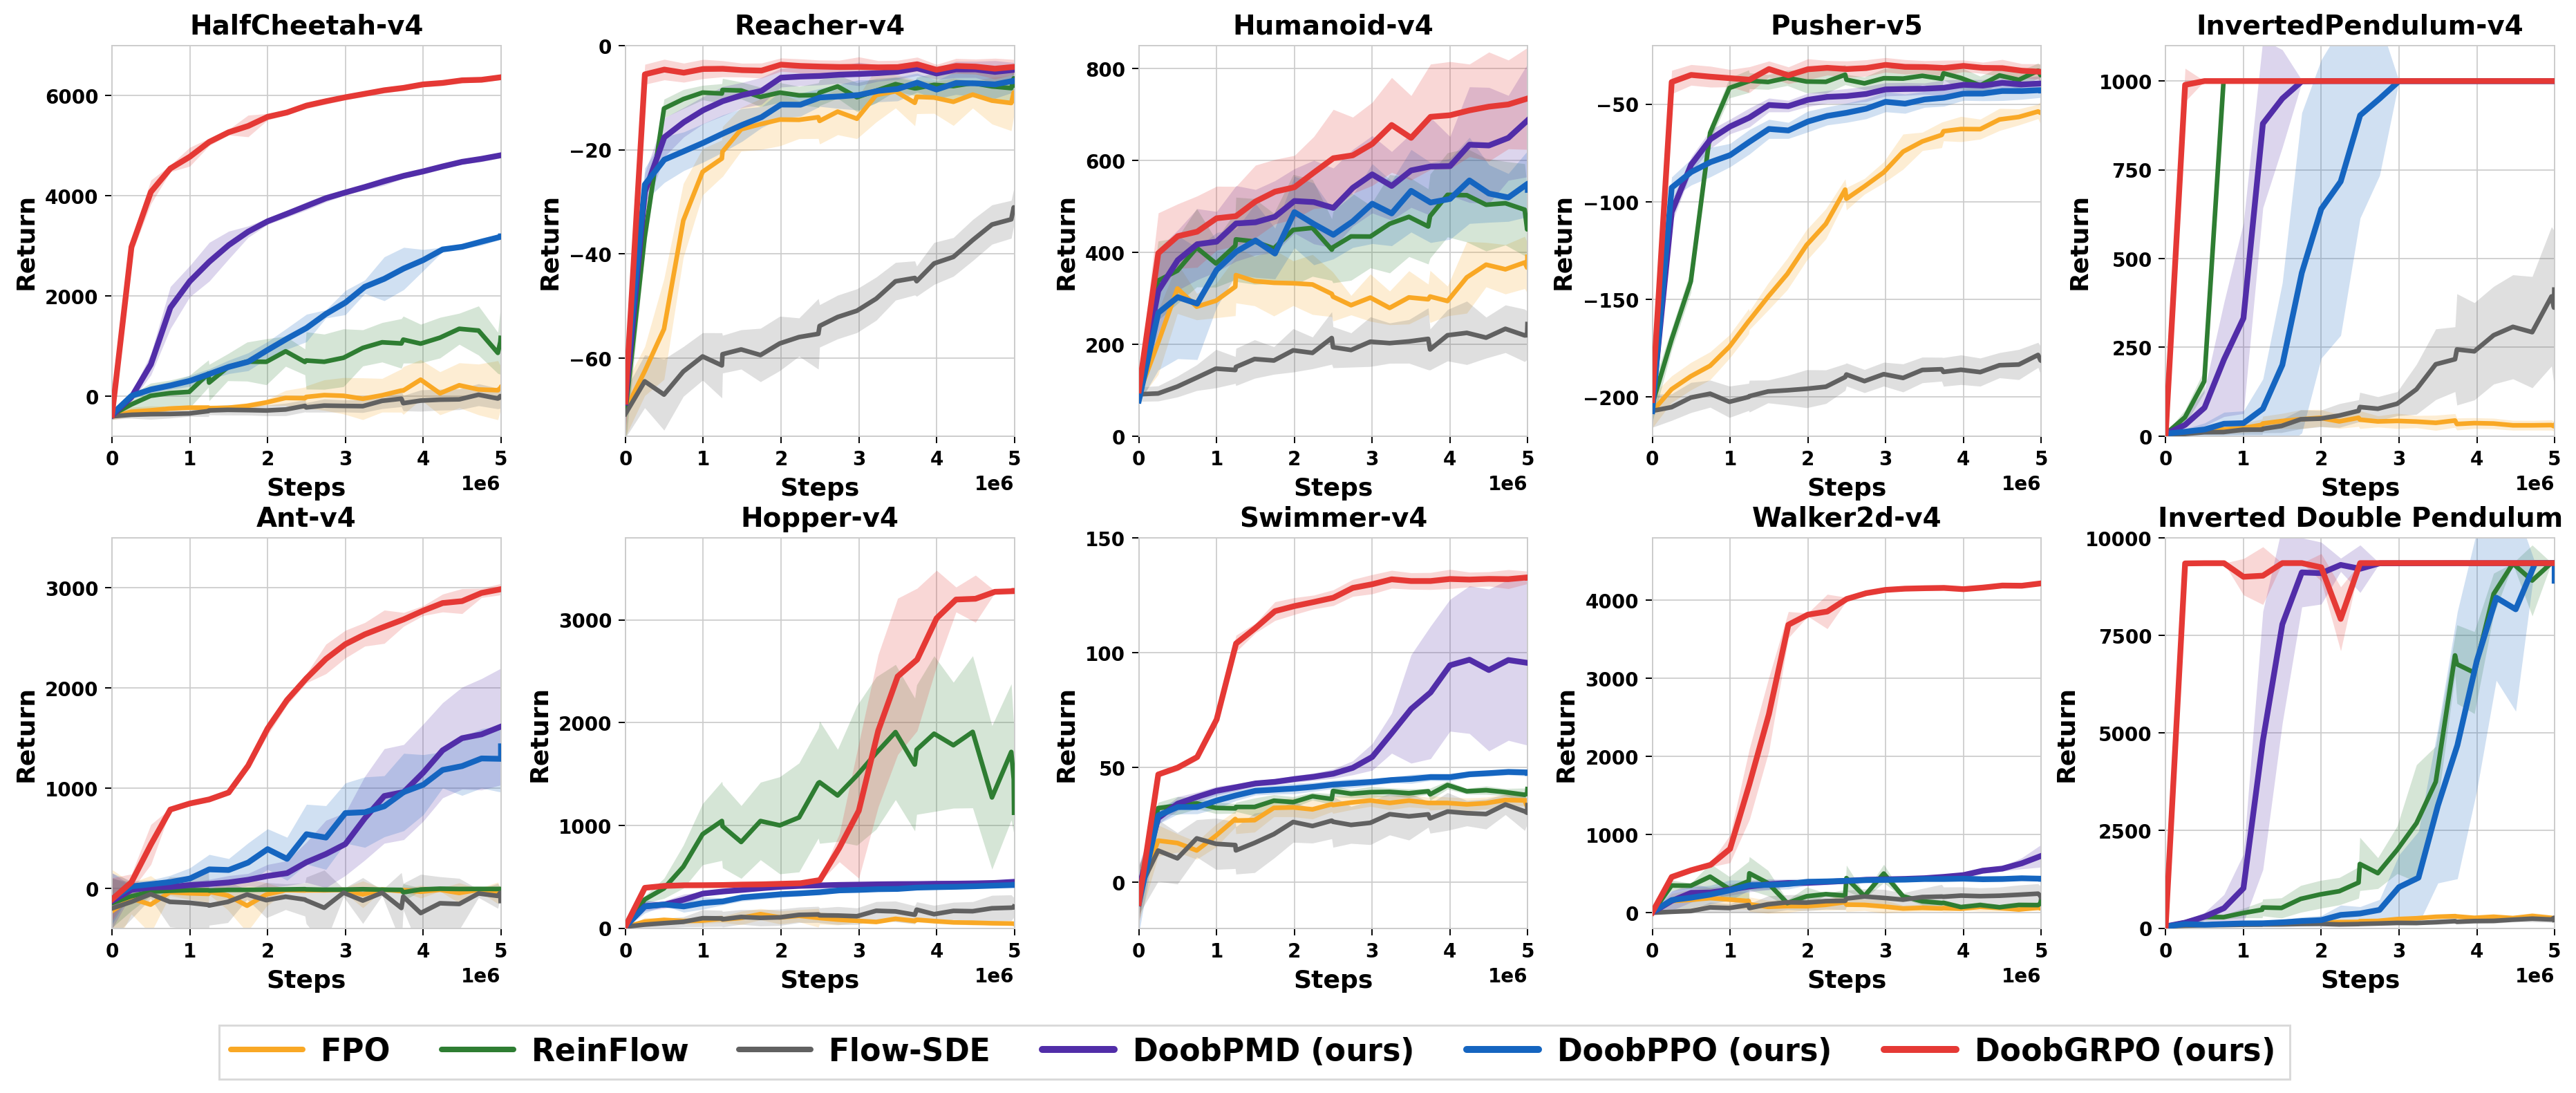
\includegraphics[width=1\linewidth]{mujoco10_flow_doob_grid.png}
    \caption{\small Learning curves on 10 MuJoCo continuous-control tasks, evaluated every 250k environment steps. Curves show mean undiscounted return over 3 training seeds, with shaded regions indicating one standard deviation. We compare DoobPO variants against flow-policy baselines FPO, ReinFlow, and Flow-SDE.}
    \label{fig:mujoco10_flow}
\end{figure}

\paragraph{Baselines.}
We compare DoobPO against three representative baselines for RL fine-tuning of flow policies: FPO \cite{mcallister2025flow}, ReinFlow \cite{zhang2025reinflow}, and Flow-SDE \cite{chen2025pirl}.
Please see \cref{sec:related_works} for more details.

\begin{table*}[t]
\centering
\small
\setlength{\tabcolsep}{3.5pt}
\renewcommand{\arraystretch}{0.95}
\caption{\small Flow Policy Performance on MuJoCo environments (mean $\pm$ std over 3 random seeds).}
\label{tab:mujoco_flow_grouped}
\begin{adjustbox}{max width=\textwidth}
\begin{tabular}{llccccc}
\toprule
& Method
& HalfCheetah
& Reacher
& Humanoid
& Pusher
& InvertedPendulum \\
\midrule

\multirow{6}{*}{\textbf{Flow Policy RL}}
& FPO
& 327 $\pm$ 399
& -8.79 $\pm$ 3.20
& 390 $\pm$ 110
& -53.77 $\pm$ 3.69
& 52 $\pm$ 24 \\

& ReinFlow
& 1344 $\pm$ 310
& -6.30 $\pm$ 2.83
& 525 $\pm$ 92
& \underline{-32.85 $\pm$ 3.81}
& \textbf{1000 $\pm$ 0} \\

& Flow-SDE
& 27 $\pm$ 219
& -31.08 $\pm$ 3.53
& 244 $\pm$ 60
& -178.42 $\pm$ 6.41
& 413 $\pm$ 238 \\

& \textbf{DoobPMD (ours)}
& \underline{4810 $\pm$ 53}
& \underline{-4.35 $\pm$ 1.40}
& \underline{688 $\pm$ 123}
& -39.10 $\pm$ 4.08
& \textbf{1000 $\pm$ 0} \\

& \textbf{DoobPPO (ours)}
& 3190 $\pm$ 60
& -6.73 $\pm$ 2.16
& 556 $\pm$ 94
& -42.81 $\pm$ 3.75
& \textbf{1000 $\pm$ 0} \\

& \textbf{DoobGRPO (ours)}
& \textbf{6368 $\pm$ 51}
& \textbf{-3.60 $\pm$ 1.37}
& \textbf{735 $\pm$ 111}
& \textbf{-29.90 $\pm$ 3.74}
& \textbf{1000 $\pm$ 0} \\

\midrule

& Method
& Ant
& Hopper
& Swimmer
& Walker2d
& Inverted2Pendulum \\
\midrule

\multirow{6}{*}{\textbf{Flow Policy RL}}
& FPO
& -13 $\pm$ 13
& 137 $\pm$ 55
& 35.8 $\pm$ 2.51
& 186 $\pm$ 140
& 314 $\pm$ 84 \\

& ReinFlow
& -5 $\pm$ 12
& \underline{1911 $\pm$ 740}
& 42.3 $\pm$ 1.77
& 503 $\pm$ 213
& \textbf{9358 $\pm$ 1} \\

& Flow-SDE
& -45 $\pm$ 41
& 210 $\pm$ 100
& 33.9 $\pm$ 4.44
& 243 $\pm$ 128
& 268 $\pm$ 68 \\

& \textbf{DoobPMD (ours)}
& \underline{1614 $\pm$ 583}
& 452 $\pm$ 4
& \underline{96.9 $\pm$ 32.13}
& \underline{726 $\pm$ 144}
& 9348 $\pm$ 0 \\

& \textbf{DoobPPO (ours)}
& 1417 $\pm$ 203
& 423 $\pm$ 10
& 48.0 $\pm$ 1.30
& 440 $\pm$ 16
& \underline{9350 $\pm$ 1} \\

& \textbf{DoobGRPO (ours)}
& \textbf{2986 $\pm$ 56}
& \textbf{3282 $\pm$ 7}
& \textbf{132.7 $\pm$ 2.71}
& \textbf{4215 $\pm$ 13}
& \underline{9350 $\pm$ 1} \\

\bottomrule
\end{tabular}
\end{adjustbox}
\end{table*}

\paragraph{Flow Policy Results.}
Table~\ref{tab:mujoco_flow_grouped} and Figure~\ref{fig:mujoco10_flow} report the flow-policy results.
Overall, DoobGRPO achieves the strongest performance across the MuJoCo benchmark under the same 5M-step training budget, obtaining the best results on 9 out of 10 tasks (including ties).
Compared with prior flow-policy RL baselines, DoobGRPO gives large gains on key locomotion tasks.
For example, it improves over the strongest baseline ReinFlow by \textbf{373.8\%} on \texttt{HalfCheetah}, \textbf{71.7\%} on \texttt{Hopper}, \textbf{213.7\%} on \texttt{Swimmer}, and \textbf{738.0\%} on \texttt{Walker2d}.
On the manipulation tasks, DoobGRPO also achieves the best performance on \texttt{Reacher} and \texttt{Pusher}, improving over ReinFlow by \textbf{42.9\%} and \textbf{9.0\%}.
DoobPMD serves as a strong second-best on several tasks, including \texttt{HalfCheetah}, \texttt{Reacher}, and \texttt{Humanoid}.
This further demonstrates the generality of the DoobPO framework across different policy-gradient methods.
These results show that DoobPO provides a useful RL framework for flow policies.

\subsection{Robomimic Manipulation}
\label{sec:robomimic_exp}

\paragraph{Setup.}
To evaluate DoobPO beyond MuJoCo continuous control, we test it on the \texttt{Can} and \texttt{Square} manipulation tasks from Robomimic \cite{mandlekar2021matters}.
Both tasks use low-dimensional state observations, sparse binary success rewards, and an action-chunk horizon of 4.
The maximum episode lengths are 300 primitive steps for \texttt{Can} and 400 for \texttt{Square}.
We follow the official Robomimic evaluation protocol with 50 parallel environments.
An episode is successful if the binary task-completion reward is achieved at least once, and the success rate is computed over all completed evaluation episodes.
We compare DoobPPO with DPPO \cite{ren2024diffusion}.
Both methods are initialized from the same pretrained diffusion behavior-cloning policy and trained for 151 iterations on \texttt{Can} and 200 iterations on \texttt{Square}, and results are averaged over 3 random seeds.
The DoobPPO hyperparameters are listed in \cref{tab:hyperparameters_robomimic}.

\paragraph{Results.}
DoobPPO matches or slightly improves upon DPPO on both tasks, reaching success rates of 99.46\% versus 99.23\% on \texttt{Can} and 99.78\% versus 99.59\% on \texttt{Square}.
Since both tasks are close to saturation, the main takeaway is not a large performance gap but that DoobPO extends to sparse-reward manipulation settings.

\subsection{Implementation Details and Ablation Studies}

Additional implementation details are provided in \cref{sec:implementation}, including computational resources, training hyperparameters, and other reproducibility details.
We also include ablation studies in \cref{sec:ablation} to examine the effect of the ratio network size and the number of sampling steps.